\documentclass[12pt]{article}

\usepackage[utf8]{inputenc}
\usepackage[T1]{fontenc}
\usepackage{mathpazo}
\usepackage{microtype}

\usepackage[a4paper, margin=1in]{geometry}
\usepackage{graphicx}
\usepackage{xcolor}
\usepackage{fancyhdr}
\usepackage{setspace}

\usepackage{amsmath,amssymb}
\usepackage{booktabs,array,tabularx}
\usepackage{enumitem}
\usepackage[font=small, labelfont=bf, textfont=it, labelsep=colon, skip=6pt]{caption}
\usepackage{subcaption}
\usepackage{titlesec}
\usepackage[titles]{tocloft}
\setlength{\cftbeforesecskip}{5pt}

\definecolor{buetmaroon}{RGB}{130,26,34}
\definecolor{titlegray}{RGB}{120,120,120}
\definecolor{subtitleblue}{RGB}{70,90,150}
\definecolor{headblue}{RGB}{44,66,128}
\definecolor{ptink}{HTML}{1F2933}
\definecolor{ptmuted}{HTML}{6A6255}
\definecolor{ptrule}{HTML}{CFC5B4}
\definecolor{ptpanel}{HTML}{F1EADE}
\definecolor{ptbg}{HTML}{FBF8F3}
\definecolor{ptgreen}{HTML}{0F7B62}
\definecolor{ptblue}{HTML}{2F5D8A}
\definecolor{ptorange}{HTML}{C2610A}
\definecolor{ptslate}{HTML}{7C8CA6}
\definecolor{ptred}{HTML}{A63446}
\definecolor{ptgold}{HTML}{B08307}


\newif\ifdrawfigures
\drawfiguresfalse

\ifdrawfigures
  \usepackage{tikz}
  \usetikzlibrary{arrows.meta,positioning,calc,fit,backgrounds,decorations.pathreplacing,shapes.geometric}
  \usepackage{pgfplots}
  \pgfplotsset{compat=1.18}
  \tikzset{
  ptnode/.style  ={rectangle, rounded corners=2.5pt, draw=ptrule, fill=white,
                   line width=0.7pt, minimum width=2.4cm, minimum height=0.9cm,
                   align=center, font=\small, text=ptink},
  ptfrozen/.style={ptnode, fill=ptpanel, draw=ptmuted!60},
  pttuned/.style ={ptnode, fill=ptgreen!12, draw=ptgreen},
  pthot/.style   ={ptnode, fill=ptorange!12, draw=ptorange},
  ptghost/.style ={ptnode, fill=ptbg, draw=ptrule, text=ptmuted},
  ptchip/.style  ={rectangle, rounded corners=1.5pt, draw=ptgreen, fill=ptgreen!18,
                   minimum width=0.5cm, minimum height=0.5cm, inner sep=0pt,
                   font=\scriptsize, text=ptink},
  ptslot/.style  ={rectangle, rounded corners=1.5pt, draw=ptmuted!70, fill=white,
                   minimum width=0.5cm, minimum height=0.5cm, inner sep=0pt,
                   font=\scriptsize, text=ptmuted},
  ptarrow/.style ={-{Stealth[length=5pt,width=4pt]}, line width=0.8pt, draw=ptmuted},
  ptgrad/.style  ={-{Stealth[length=5pt,width=4pt]}, line width=1.0pt, draw=ptgreen,
                   dash pattern=on 3pt off 2pt},
  ptlbl/.style   ={font=\footnotesize, text=ptmuted, align=center},
  ptlblg/.style  ={font=\footnotesize\bfseries, text=ptgreen, align=center},
}

\newcommand{\ptsnow}[1]{%
  \begin{scope}[shift={#1}]
    \foreach \a in {0,60,120}{%
      \draw[line width=0.7pt, draw=ptblue] (\a:0.14) -- (\a+180:0.14);}
  \end{scope}}


\newcommand{\figservingcompare}{%
\begin{tikzpicture}
  \node[font=\small\bfseries, text=ptorange] at (2.2,2.3) {Model tuning};
  \foreach \t/\y in {A/1.25, B/0, C/-1.25}{
    \node[ptghost, minimum width=1.5cm, minimum height=0.75cm, font=\footnotesize]
      (b\t) at (0.55,\y) {Task \t\\[-3pt]batch};
    \node[pthot, minimum width=2.6cm, minimum height=0.8cm, font=\footnotesize]
      (m\t) at (3.5,\y) {Task \t{} model\\[-3pt]11B parameters};
    \draw[ptarrow] (b\t.east) -- (m\t.west);
  }
  \node[ptlbl, anchor=north] at (2.2,-1.85)
    {one model copy and\\one batch per task};
  \draw[ptrule, dashed, line width=0.8pt] (5.4,-2.75) -- (5.4,2.55);
  \node[font=\small\bfseries, text=ptgreen] at (8.6,2.3) {Prompt tuning};
  \node[ptghost, minimum width=2.1cm, minimum height=2.9cm] (mix) at (6.95,0) {};
  \foreach \t/\y/\col in {A/0.9/ptgreen, C/0.3/ptgold, B/-0.3/ptblue, A/-0.9/ptgreen}{
    \node[rectangle, rounded corners=1.2pt, draw=\col, fill=\col!20,
          minimum width=0.45cm, minimum height=0.4cm, inner sep=0pt,
          font=\scriptsize\bfseries, text=\col] at (6.4,\y) {\t};
    \node[rectangle, rounded corners=1.2pt, draw=ptmuted!60, fill=white,
          minimum width=1.05cm, minimum height=0.4cm, inner sep=0pt,
          font=\scriptsize, text=ptmuted] at (7.25,\y) {input};
  }
  \node[ptfrozen, minimum width=2.7cm, minimum height=2.9cm, font=\footnotesize]
       (fm) at (10.25,0)
       {Pretrained model\\11B parameters\\[3pt]\textbf{frozen, shared}};
  \ptsnow{(10.25,-1.05)}
  \draw[ptarrow] (mix.east) -- (fm.west);
  \node[ptlbl, anchor=north] at (6.95,-1.5) {mixed-task batch};
  \node[ptlbl, anchor=north] at (8.75,-2.05)
    {one shared model; each task adds only its\\
     prompt ($20{,}480$ parameters when $m=5$)};
\end{tikzpicture}}


\newcommand{\figanalogy}{%
\begin{tikzpicture}
  \node[ptnode, text width=4.6cm, minimum height=2.0cm, align=left, font=\small]
       (a) at (0,0)
       {Classify the sentiment of this movie review as \emph{positive} or \emph{negative}:};
  \node[ptlbl, anchor=south] at (a.north) {hard prompt: text a person writes};
  \node[pttuned, minimum height=2.0cm, font=\scriptsize] (b) at (7.1,0)
       {\renewcommand{\arraystretch}{1.25}%
        \begin{tabular}{@{}l@{\hspace{8pt}}rrrr@{}}
          $p_1$ & $0.14$ & $-0.72$ & $0.31$ & $0.08$\\
          $p_2$ & $-0.45$ & $0.19$ & $0.66$ & $-0.27$\\
          $p_3$ & $0.52$ & $-0.11$ & $0.03$ & $0.94$
        \end{tabular}};
  \node[ptlblg, anchor=south] at (b.north) {soft prompt: vectors training learns};
  \draw[ptarrow] (a.east) -- (b.west) node[midway, above, ptlbl] {replaced by};
\end{tikzpicture}}


\newcommand{\figarchitecture}{%
\begin{tikzpicture}
  \node[ptfrozen, minimum width=8.2cm, minimum height=1.35cm, font=\small]
       (lm) at (0.4,2.5)
       {Pretrained Transformer $f_\theta$\\[1pt]
        {\footnotesize\bfseries frozen: the weights $\theta$ are never updated}};
  \ptsnow{(4.1,2.5)}
  \node[ptnode, minimum width=4.2cm, minimum height=0.7cm, font=\footnotesize]
       (out) at (0.4,4.25) {output $Y$, scored against the target};
  \draw[ptarrow] (lm.north) -- (out.south);
  \foreach \i in {1,...,4}{
    \node[ptchip, minimum width=0.62cm, minimum height=0.62cm]
         (p\i) at ({-3.7+0.8*\i},0.55) {$p_{\i}$};}
  \foreach \i/\w in {1/The, 2/movie, 3/was, 4/great}{
    \node[ptslot, minimum width=0.62cm, minimum height=0.62cm]
         (x\i) at ({0.8+0.8*\i},0.55) {};
    \node[font=\scriptsize\itshape, text=ptmuted] (w\i) at ({0.8+0.8*\i},-0.45) {\w};
    \draw[ptarrow, line width=0.5pt] (w\i.north) -- (x\i.south);
  }
  \node[draw=ptgreen, rounded corners=3pt, dashed, fit=(p1)(p4), inner sep=4pt] (P) {};
  \node[draw=ptmuted!70, rounded corners=3pt, dashed, fit=(x1)(x4), inner sep=4pt] (X) {};
  \node[ptlblg, anchor=north] at (-1.7,-0.1)
       {soft prompt $P\in\mathbb{R}^{m\times d}$\\[-1pt]{\normalfont trainable}};
  \node[ptlbl, anchor=north] at (2.8,-0.75)
       {input embeddings $E(X)\in\mathbb{R}^{n\times d}$\\[-1pt]frozen lookup};
  \draw[ptarrow] (P.north) -- (P.north |- lm.south);
  \draw[ptarrow] (X.north) -- (X.north |- lm.south);
  \node[ptlbl, fill=white, inner sep=1.5pt] at (0.55,1.38)
       {$[P;E(X)]\in\mathbb{R}^{(m+n)\times d}$};
  \draw[ptgrad] (out.west) -- (-4.55,4.25) -- (-4.55,0.55) -- (P.west);
  \node[ptlblg, rotate=90, anchor=south] at (-4.55,2.4) {gradient $\nabla_P\mathcal{L}$};
\end{tikzpicture}}


\newcommand{\figparams}{%
\begin{tikzpicture}
\begin{axis}[
  width=12.2cm, height=6.6cm,
  xmode=log, ymode=log,
  xmin=5e7, xmax=2.4e10, ymin=1e3, ymax=3e11,
  xtick={76961152,247577856,783150080,2849757184,11135332352},
  xticklabels={Small\\77M, Base\\248M, Large\\783M, XL\\2.85B, XXL\\11.1B},
  xticklabel style={align=center, font=\scriptsize},
  yticklabel style={font=\scriptsize},
  ytick={1e3,1e5,1e7,1e9,1e11},
  xlabel={T5.1.1 model size (frozen parameters)},
  ylabel={task-specific parameters},
  label style={font=\footnotesize},
  axis line style={draw=ptmuted!70},
  tick style={draw=ptmuted!70},
  grid=major, grid style={draw=ptrule!70, dashed, line width=0.3pt},
  legend style={at={(0.5,1.03)}, anchor=south, draw=none, fill=none,
                font=\scriptsize, /tikz/every even column/.append style={column sep=10pt}},
  legend columns=3,
  legend cell align=left,
  clip=false,
]
  \addplot[ptorange, line width=1.3pt, mark=square*, mark size=1.8pt] coordinates
    {(76961152,76961152) (247577856,247577856) (783150080,783150080)
     (2849757184,2849757184) (11135332352,11135332352)};
  \addlegendentry{Model tuning (all weights)}
  \addplot[ptgreen, line width=1.3pt, mark=*, mark size=1.8pt] coordinates
    {(76961152,51200) (247577856,76800) (783150080,102400)
     (2849757184,204800) (11135332352,409600)};
  \addlegendentry{Prompt tuning, $m=100$ (default)}
  \addplot[ptgreen, line width=1.2pt, dashed, mark=o, mark size=1.8pt,
           mark options={solid, fill=white}] coordinates
    {(76961152,2560) (247577856,3840) (783150080,5120)
     (2849757184,10240) (11135332352,20480)};
  \addlegendentry{Prompt tuning, $m=5$}
  \draw[{Stealth[length=4pt]}-{Stealth[length=4pt]}, ptmuted, line width=0.7pt]
       (axis cs:1.55e10,409600) -- (axis cs:1.55e10,11135332352)
       node[midway, right, font=\scriptsize, text=ptink, align=left]
       {$\approx 27{,}000\times$\\fewer};
\end{axis}
\end{tikzpicture}}


\newcommand{\figworkflow}{%
\begin{tikzpicture}[font=\footnotesize]
  \node[ptghost, text=ptink, minimum width=2.7cm, minimum height=0.8cm, font=\footnotesize]
       (s1) at (0,1.2) {\textbf{1} Define the task\\[-2pt]and labeled data};
  \node[pttuned, minimum width=2.7cm, minimum height=0.8cm, font=\footnotesize]
       (s2) at (0,0) {\textbf{2} Initialize the\\[-2pt]soft prompt $P$};
  \node[ptfrozen, minimum width=2.7cm, minimum height=0.8cm, font=\footnotesize]
       (s3) at (0,-1.2) {\textbf{3} Freeze the\\[-2pt]model weights $\theta$};
  \draw[ptarrow] (s1) -- (s2);
  \draw[ptarrow] (s2) -- (s3);
  \node[draw=ptrule, rounded corners=6pt, dashed, fit=(s1)(s2)(s3), inner sep=6pt,
        label={[ptlbl]above:setup}] (setup) {};
  \node[ptnode, minimum width=2.8cm, minimum height=0.8cm, font=\footnotesize]
       (s4) at (4.2,0.95) {\textbf{4} Forward pass\\[-2pt]on $[P;E(X)]$};
  \node[ptnode, minimum width=2.8cm, minimum height=0.8cm, font=\footnotesize]
       (s5) at (7.7,0.95) {\textbf{5} Cross-entropy\\[-2pt]loss $\mathcal{L}$};
  \node[ptnode, minimum width=2.8cm, minimum height=0.8cm, font=\footnotesize]
       (s6) at (7.7,-0.95) {\textbf{6} Backpropagate\\[-2pt]to get $\nabla_P\mathcal{L}$};
  \node[pttuned, minimum width=2.8cm, minimum height=0.8cm, font=\footnotesize]
       (s7) at (4.2,-0.95) {\textbf{7} Update $P$ only\\[-2pt]$P\leftarrow P-\eta\nabla_P\mathcal{L}$};
  \draw[ptarrow] (s4) -- (s5);
  \draw[ptarrow] (s5) -- (s6);
  \draw[ptgrad]  (s6) -- (s7);
  \draw[ptarrow] (s7) -- (s4);
  \node[ptlbl, font=\scriptsize] at (5.95,0) {repeat for\\[-2pt]each mini-batch};
  \node[draw=ptrule, rounded corners=6pt, dashed, fit=(s4)(s5)(s6)(s7), inner sep=6pt,
        label={[ptlbl]above:training loop}] (loop) {};
  \draw[ptarrow] (setup.east) -- (loop.west);
  \node[pttuned, minimum width=2.4cm, minimum height=1.2cm, font=\footnotesize]
       (s8) at (12.4,0) {\textbf{8} Store the task\\[-2pt]prompt $P^{\star}$\\[-2pt](kilobytes)};
  \draw[ptarrow] (loop.east) -- (s8.west)
       node[midway, above=1pt, ptlbl, font=\scriptsize] {converged};
\end{tikzpicture}}


\newcommand{\figexampleforward}{%
\begin{tikzpicture}
  \foreach \i in {1,2,3}{
    \node[ptchip, minimum width=0.6cm, minimum height=0.6cm]
         (p\i) at ({-3.0+0.72*(\i-1)},3.3) {$p_{\i}$};}
  \node[ptghost, minimum height=0.6cm, minimum width=0pt, inner xsep=5pt, font=\footnotesize]
       (inp) at (1.15,3.3) {``The movie was fantastic.''};
  \node[ptfrozen, minimum width=5.4cm, minimum height=0.9cm, font=\small]
       (lm) at (-0.3,2.0) {Frozen model $f_\theta$};
  \ptsnow{(2.05,2.0)}
  \draw[ptarrow] (-0.3,2.97) -- (lm.north);
  \draw[ptarrow] (lm.south) -- (-0.3,1.12);
  \node[anchor=east, font=\footnotesize] at (-1.6,0.8) {Positive};
  \fill[ptgreen!40] (-1.5,0.62) rectangle ++(1.4,0.36);
  \draw[ptgreen, line width=0.6pt] (-1.5,0.62) rectangle ++(1.4,0.36);
  \node[anchor=west, font=\footnotesize] at (-0.05,0.8)
       {$0.40$ \textcolor{ptgreen}{(target)}};
  \node[anchor=east, font=\footnotesize] at (-1.6,0.25) {Negative};
  \fill[ptred!35] (-1.5,0.07) rectangle ++(2.1,0.36);
  \draw[ptred, line width=0.6pt] (-1.5,0.07) rectangle ++(2.1,0.36);
  \node[anchor=west, font=\footnotesize] at (0.65,0.25)
       {$0.60$ \textcolor{ptred}{(predicted)}};
  \draw[ptmuted!60] (-1.5,-0.05) -- (-1.5,1.1);
  \draw[ptgrad] (3.0,0.53) -- (3.55,0.53) -- (3.55,4.15) -- (p2.north |- 0,4.15) -- (p2.north);
  \node[ptlblg, anchor=south] at (0.3,4.15) {$\nabla_P\mathcal{L}$ flows back to $P$ only};
\end{tikzpicture}}


\newcommand{\figlosscurve}{%
\begin{tikzpicture}
\begin{axis}[
  width=6.4cm, height=5.4cm,
  xmin=0, xmax=1.05, ymin=0, ymax=3.2,
  xlabel={probability of the correct class, $q$},
  ylabel={loss $\mathcal{L}=-\ln q$},
  xtick={0,0.2,0.4,0.6,0.8,1.0},
  ytick={0,1,2,3},
  axis lines=left,
  axis line style={draw=ptmuted!70},
  tick style={draw=ptmuted!70},
  tick label style={font=\scriptsize},
  label style={font=\footnotesize},
  grid=major, grid style={draw=ptrule!70, dashed, line width=0.3pt},
  clip=false,
]
  \addplot[domain=0.045:1, samples=150, line width=1.3pt, color=ptblue] {-ln(x)};
  \addplot[only marks, mark=*, mark size=2.3pt, color=ptred]
    coordinates {(0.40,0.9163)};
  \node[anchor=south west, font=\scriptsize, text=ptred]
    at (axis cs:0.42,1.0) {$q=0.40$: $\mathcal{L}\approx0.916$};
  \addplot[only marks, mark=o, mark size=2.3pt, color=ptmuted, thick]
    coordinates {(0.5,0.6931)};
  \node[anchor=west, font=\scriptsize, text=ptmuted]
    at (axis cs:0.55,0.74) {chance: $\mathcal{L}\approx0.693$};
  \addplot[only marks, mark=*, mark size=2.3pt, color=ptgreen]
    coordinates {(1,0)};
  \node[anchor=south, font=\scriptsize, text=ptgreen]
    at (axis cs:1.0,0.1) {$\mathcal{L}=0$};
\end{axis}
\end{tikzpicture}}


\tikzset{
  stklayer/.style ={rectangle, rounded corners=1.5pt, draw=ptmuted!60, fill=ptpanel,
                    minimum width=2.7cm, minimum height=0.5cm, font=\scriptsize, text=ptink},
  stkhot/.style   ={stklayer, draw=ptorange, fill=ptorange!18},
  stkright/.style ={stklayer, text width=2.45cm, align=right},
  stkadapt/.style ={rectangle, rounded corners=1pt, draw=ptgreen, fill=ptgreen!30,
                    minimum width=1.2cm, minimum height=0.2cm, inner sep=0pt},
  stktok/.style   ={rectangle, rounded corners=1pt, draw=ptmuted!60, fill=white,
                    minimum width=0.28cm, minimum height=0.28cm, inner sep=0pt},
  stkgtok/.style  ={stktok, draw=ptgreen, fill=ptgreen!35},
}
\newcommand{\ptstack}[3]{%
  \node[#2] at (#1,3.05) {Layer $L$};
  \node[text=ptmuted, font=\small] at (#1,2.38) {$\vdots$};
  \node[#2] at (#1,1.65) {Layer 2};
  \node[#2] at (#1,0.8)  {Layer 1};
  \foreach \k in {0,...,6}{%
    \ifnum\k<#3\relax
      \node[stkgtok] at ({#1-1.02+0.34*\k},0.02) {};
    \else
      \node[stktok]  at ({#1-1.02+0.34*\k},0.02) {};
    \fi}
  \draw[ptarrow, line width=0.5pt] (#1,0.2) -- (#1,0.53);
}
\newcommand{\figpeftstack}{%
\begin{tikzpicture}
  \node[font=\footnotesize\bfseries, text=ptorange] at (0,3.95) {Full fine-tuning};
  \ptstack{0}{stkhot}{0}
  \node[font=\footnotesize\bfseries] at (3.8,3.95) {Adapters};
  \ptstack{3.8}{stklayer}{0}
  \foreach \y in {1.225,2.075,3.475}{\node[stkadapt] at (3.8,\y) {};}
  \node[font=\footnotesize\bfseries] at (7.6,3.95) {Prefix tuning};
  \ptstack{7.6}{stkright}{3}
  \foreach \y in {0.8,1.65,3.05}{
    \foreach \k in {0,1,2}{\node[stkgtok] at ({7.6-1.1+0.32*\k},\y) {};}}
  \node[font=\footnotesize\bfseries, text=ptgreen] at (11.4,3.95) {Prompt tuning};
  \ptstack{11.4}{stklayer}{3}
  \foreach \x/\s in {0/{100\%}, 3.8/{2--4\%}, 7.6/{0.1--1\%}, 11.4/{${<}\,0.01\%$}}{
    \node[font=\footnotesize, text=ptink] at (\x,-0.55) {task-specific: \textbf{\s}};}
  \node[stkhot, minimum width=0.45cm, minimum height=0.3cm] at (1.3,-1.25) {};
  \node[anchor=west, font=\scriptsize, text=ptmuted] at (1.6,-1.25) {trained (all weights)};
  \node[stkgtok, minimum width=0.45cm, minimum height=0.3cm] at (5.0,-1.25) {};
  \node[anchor=west, font=\scriptsize, text=ptmuted] at (5.3,-1.25) {trained, task-specific};
  \node[stklayer, minimum width=0.45cm, minimum height=0.3cm] at (8.7,-1.25) {};
  \node[anchor=west, font=\scriptsize, text=ptmuted] at (9.0,-1.25) {frozen, shared};
\end{tikzpicture}}


\newcommand{\figtaxonomy}{%
\begin{tikzpicture}[
   txroot/.style  ={ptnode, fill=ptink, draw=ptink, text=white, minimum width=2.3cm,
                    minimum height=0.95cm, font=\footnotesize\bfseries},
   txdirect/.style={pttuned, minimum width=2.5cm, minimum height=0.8cm, font=\footnotesize\bfseries},
   txtrans/.style ={ptnode, fill=ptblue!12, draw=ptblue, minimum width=2.5cm,
                    minimum height=0.8cm, font=\footnotesize\bfseries},
   txcat/.style   ={ptnode, minimum width=3.0cm, minimum height=0.55cm, font=\footnotesize},
   txleaf/.style  ={anchor=west, font=\footnotesize, text=ptink},
   txedge/.style  ={draw=ptmuted!80, line width=0.7pt}]
  \node[txroot] (r) at (0,-0.35) {Prompt-tuning\\methods};
  \node[txdirect] (d) at (3.2,1.6) {Direct prompt\\learning};
  \node[txtrans]  (t) at (3.2,-2.3) {Transfer\\learning};
  \draw[txedge] (r.east) -- ++(0.3,0) |- (d.west);
  \draw[txedge] (r.east) -- ++(0.3,0) |- (t.west);
  \node[ptlbl, font=\scriptsize, anchor=north] at (3.2,1.1) {one training stage\\on the target task};
  \node[ptlbl, font=\scriptsize, anchor=north] at (3.2,-2.8) {reuse prompts learned\\on source tasks};
  \node[txcat] (dg) at (6.55,3.1)  {General};
  \node[txcat] (de) at (6.55,2.1)  {Encoder-based};
  \node[txcat] (dd) at (6.55,1.1)  {Decomposition};
  \node[txcat] (dm) at (6.55,0.1)  {Mixture of experts};
  \foreach \n in {dg,de,dd,dm}{\draw[txedge] (d.east) -- ++(0.3,0) |- (\n.west);}
  \node[txleaf] at (8.2,3.1)  {Prompt Tuning, XPrompt, P-Tuning v2};
  \node[txleaf] at (8.2,2.1)  {P-Tuning, Residual PT, Prefix Tuning};
  \node[txleaf] at (8.2,1.1)  {DPT, DePT};
  \node[txleaf] at (8.2,0.1)  {SMoP, PT-MoE};
  \node[txcat] (tg) at (6.55,-1.3) {General};
  \node[txcat] (te) at (6.55,-2.3) {Encoder-based};
  \node[txcat] (td) at (6.55,-3.3) {Decomposition};
  \foreach \n in {tg,te,td}{\draw[txedge] (t.east) -- ++(0.3,0) |- (\n.west);}
  \node[txleaf] at (8.2,-1.3) {SPoT, ATTEMPT};
  \node[txleaf] at (8.2,-2.3) {TransPrompt, CTPT};
  \node[txleaf] at (8.2,-3.3) {MPT};
\end{tikzpicture}}


\newcommand{\figspectrum}{%
\begin{tikzpicture}
  \draw[ptrule, line width=1.4pt, -{Stealth[length=7pt]}] (0,0) -- (11.2,0);
  \foreach \x/\lbl/\col/\sub in {
      0.6/{Prompt\\engineering}/ptslate/{write the prompt\\by hand},
      5.6/{Prompt\\tuning}/ptgreen/{learn a few vectors,\\freeze the model},
      10.6/{Full\\fine-tuning}/ptorange/{update every\\weight}}{
    \fill[\col] (\x,0) circle (3.5pt);
    \node[font=\small\bfseries, text=\col, align=center] at (\x,0.8) {\lbl};
    \node[ptlbl, font=\scriptsize] at (\x,-0.7) {\sub};
  }
  \node[ptlbl, font=\scriptsize] at (5.6,-1.55)
    {$\longleftarrow$ faster and cheaper \hspace{2.2cm} more control, more cost $\longrightarrow$};
\end{tikzpicture}}


\newcommand{\figradar}{%
\begin{tikzpicture}
  \def\R{2.0}
  \foreach \r in {1,2,3}{\draw[ptrule, dashed, line width=0.4pt] (0,0) circle ({\r*\R/3});}
  \foreach \ang in {90,18,-54,-126,162}{\draw[ptrule, line width=0.6pt] (0,0) -- (\ang:\R);}
  \node[ptlbl, anchor=south] at (90:{\R+0.12}) {Speed of implementation};
  \node[ptlbl, anchor=west, align=left] at (18:{\R+0.15}) {Data\\requirement};
  \node[ptlbl, anchor=north west, align=left] at (-54:{\R+0.08}) {Output\\quality};
  \node[ptlbl, anchor=north east, align=right] at (-126:{\R+0.08}) {Model\\modification};
  \node[ptlbl, anchor=east, align=right] at (162:{\R+0.15}) {Flexibility};
  \draw[ptorange, line width=1.3pt, fill=ptorange, fill opacity=0.14]
    (90:{3/9*\R}) -- (18:{9/9*\R}) -- (-54:{8/9*\R}) -- (-126:{8/9*\R})
    -- (162:{5/9*\R}) -- cycle;
  \draw[ptgreen, line width=1.3pt, fill=ptgreen, fill opacity=0.16]
    (90:{8/9*\R}) -- (18:{2/9*\R}) -- (-54:{4/9*\R}) -- (-126:{1/9*\R})
    -- (162:{7/9*\R}) -- cycle;
  \fill[ptorange, fill opacity=0.3] (4.3,0.55) rectangle ++(0.45,0.3);
  \draw[ptorange, line width=1pt] (4.3,0.55) rectangle ++(0.45,0.3);
  \node[anchor=west, font=\footnotesize] at (4.85,0.7) {Full fine-tuning};
  \fill[ptgreen, fill opacity=0.3] (4.3,-0.05) rectangle ++(0.45,0.3);
  \draw[ptgreen, line width=1pt] (4.3,-0.05) rectangle ++(0.45,0.3);
  \node[anchor=west, font=\footnotesize] at (4.85,0.1) {Prompt tuning};
\end{tikzpicture}}

\else
  \newcommand{\figpage}[1]{\includegraphics[page=#1]{all-figures.pdf}}
  \newcommand{\figservingcompare}{\figpage{1}}
  \newcommand{\figanalogy}{\figpage{2}}
  \newcommand{\figarchitecture}{\figpage{3}}
  \newcommand{\figparams}{\figpage{4}}
  \newcommand{\figworkflow}{\figpage{5}}
  \newcommand{\figexampleforward}{\figpage{6}}
  \newcommand{\figlosscurve}{\figpage{7}}
  \newcommand{\figpeftstack}{\figpage{8}}
  \newcommand{\figtaxonomy}{\figpage{9}}
  \newcommand{\figspectrum}{\figpage{10}}
  \newcommand{\figradar}{\figpage{11}}
\fi

\usepackage[colorlinks=true, linkcolor=headblue, citecolor=ptgreen,
            urlcolor=headblue]{hyperref}
\hypersetup{pdftitle={Prompt Tuning: A Study on Task-Specific Prompt Learning},
            pdfauthor={Sk. Arib Rajin Shahan, Sadman Zaman, Fatin Nehal Zubaeer},
            pdfsubject={CSE 200 report on parameter-efficient prompt tuning}}
\usepackage{algorithm}
\usepackage{algpseudocode}
\algrenewcommand\algorithmicrequire{\textbf{Input:}}
\algrenewcommand\algorithmicensure{\textbf{Output:}}

\titleformat{\section}{\normalfont\Large\bfseries\color{headblue}}{\thesection.}{0.5em}{}
            [\nobreak\vspace{1pt}{\color{ptrule}\nobreak\titlerule[0.6pt]}\nobreak]%
\titleformat{\subsection}{\normalfont\large\bfseries\color{headblue}}{\thesubsection.}{0.5em}{}
\titleformat{\subsubsection}{\normalfont\normalsize\bfseries\color{buetmaroon}}{\thesubsubsection.}{0.5em}{}
\titlespacing*{\section}{0pt}{18pt plus 4pt minus 2pt}{9pt plus 2pt}
\titlespacing*{\subsection}{0pt}{13pt plus 3pt minus 2pt}{6pt plus 2pt}

\newcounter{definition}
\newsavebox{\defbody}
\newenvironment{definition}[2]{%
  \par\addvspace{10pt}%
  \refstepcounter{definition}\label{def:#2}%
  \gdef\deftitle{Definition~\thedefinition: #1}%
  \begin{lrbox}{\defbody}%
  \begin{minipage}{\dimexpr\linewidth-19.2pt\relax}%
}{%
  \end{minipage}%
  \end{lrbox}%
  \noindent{\setlength{\fboxsep}{0pt}\setlength{\fboxrule}{0.6pt}%
  \fcolorbox{buetmaroon}{buetmaroon!3}{%
    \begin{minipage}{\dimexpr\linewidth-1.2pt\relax}%
      \colorbox{buetmaroon}{\makebox[\linewidth][l]{%
        \hspace{9pt}\rule[-5pt]{0pt}{17pt}\small\bfseries\color{white}\deftitle}}\par
      \kern6pt\hspace*{9pt}\usebox{\defbody}\par\kern6pt%
    \end{minipage}}}%
  \par\addvspace{10pt}%
}

\renewcommand{\topfraction}{0.85}
\renewcommand{\bottomfraction}{0.6}
\renewcommand{\textfraction}{0.15}
\renewcommand{\floatpagefraction}{0.75}

\renewcommand{\arraystretch}{1.25}
\newcolumntype{L}{>{\raggedright\arraybackslash}X}
\setlist{itemsep=2pt, topsep=4pt}

\newcommand{\R}{\mathbb{R}}
\newcommand{\loss}{\mathcal{L}}
\newcommand{\data}{\mathcal{D}}
\newcommand{\PrTP}{\Pr\nolimits_{\theta;P}}

\setstretch{1.1}

\setlength{\headheight}{14.5pt}
\pagestyle{fancy}
\fancyhf{}
\renewcommand{\headrulewidth}{0.4pt}
\fancyhead[L]{\small CSE 200 --- BUET}
\fancyhead[R]{\small Prompt Tuning}
\fancyfoot[C]{\thepage}

\fancypagestyle{plain}{%
  \fancyhf{}
  \renewcommand{\headrulewidth}{0.4pt}
  \fancyhead[L]{\small CSE 200 --- BUET}
  \fancyhead[R]{\small Prompt Tuning}
  \fancyfoot[C]{\thepage}
}

\begin{document}

\hypersetup{pageanchor=false}
\begin{titlepage}
\thispagestyle{empty}
\centering

\vspace*{1.2cm}

{
\includegraphics[width=4.0cm]{buet_logo.png}}

\vspace{0.6cm}

{\scshape\large \textcolor{titlegray}{Bangladesh University of Engineering and Technology}}\\[2pt]
{\scshape\large \textcolor{titlegray}{Department of Computer Science and Engineering}}

\vspace{0.8cm}
{\color{buetmaroon}\rule{0.35\textwidth}{1.2pt}}
\vspace{1.0cm}

{\Large\bfseries Prompt Tuning}

\vspace{0.9cm}

{\large\itshape\color{subtitleblue} A Study on Task-Specific Prompt Learning}

\vspace{1.0cm}
{\color{buetmaroon}\rule{0.35\textwidth}{1.2pt}}
\vspace{1.2cm}

\begin{tabular}{ccc}
\textbf{Sk Arib Rajin Shahan} & \textbf{Sadman Zaman} & \textbf{Fatin Nehal Zubaeer}\\[2pt]
\textit{2305068} & \textit{2305075} & \textit{2305076}
\end{tabular}

\vspace{1.0cm}

{\small CSE 200: Technical Writing and Presentation}

\vspace{0.4cm}

{\small September 23, 2026}

\vfill
\end{titlepage}
\hypersetup{pageanchor=true}

\newpage
\thispagestyle{plain}

\section*{Abstract}

Large pretrained language models are usually adapted to a new task by fine-tuning all of
their weights, which leaves one full copy of the model for every task. Prompt tuning avoids
this cost. It keeps the model frozen and learns only a short sequence of continuous vectors,
called a \emph{soft prompt}, that is placed in front of the input. In this report we explain
how prompt tuning works and when it is worth using. We define the method mathematically and
show that a prompt of $m$ tokens for a model with embedding dimension $d$ adds only $m\cdot d$
trained parameters per task. For the 11-billion-parameter T5-XXL model with a 100-token
prompt this comes to 409,600 parameters, or 0.0037\% of the model. We then follow one gradient step
on a small sentiment task by hand to show how the loss is computed and why only the prompt
changes. The experiments of Lester et al.\ show that prompt tuning catches up with full
fine-tuning as models grow, that it transfers better to new domains (by up to 12.5 F1
points), and that it makes ensembles cheap. We also compare the method with related
parameter-efficient techniques, suggest when to prefer it over fine-tuning, and discuss the
problems that remain open, namely slow training, sensitivity to initialization, weak results
on small models, and prompts that people cannot read.

\vspace{0.8em}
\noindent\textbf{Keywords:} prompt tuning; soft prompts; parameter-efficient fine-tuning;
large language models; transfer learning.

\newpage
{\setstretch{1.0}\tableofcontents}
\newpage

\section{Introduction}\label{sec:intro}

Large language models learn a great deal about language during pretraining, but most real
applications need them to do one specific job well, such as classifying reviews or
answering questions. The usual way to specialize a model is \emph{model tuning}, also called
full fine-tuning, which updates every weight of the network on labeled data for the
task~\cite{lester2021}. Model tuning works well, but it becomes expensive as models grow. A
tuned copy of T5-XXL~\cite{raffel2020} holds 11 billion parameters and takes about 42\,GiB of
storage, and every new task needs a copy of its own~\cite{lester2021}.

Prompt design takes the opposite route. The model stays unchanged, and the user describes the
task in the input text instead. Brown et al.~\cite{brown2020} showed that a frozen GPT-3 can solve
new tasks when its prompt contains an instruction and a few examples. Hand-written prompts
are fragile, however, and they can hold only as much text as the input allows. Few-shot
GPT-3 with 175 billion parameters scores 71.8 on the SuperGLUE
benchmark~\cite{wang2019superglue}, while a fine-tuned T5-XXL scores 89.3 with 16 times fewer
parameters~\cite{lester2021}.

Prompt tuning~\cite{lester2021} borrows one idea from each approach. It keeps the model
frozen, as prompt design does, and it learns the task from labeled data by gradient descent,
as fine-tuning does. We use the following definition throughout the report.

\begin{definition}{Prompt tuning}{prompttuning}
Prompt tuning is a parameter-efficient adaptation method. It freezes every weight of a
pretrained language model and trains only a short sequence of continuous vectors, the
\emph{soft prompt}, which is prepended to the embedded input of every example.
\end{definition}

Since the prompt is learned, it can absorb the information in a whole labeled dataset rather
than the few examples that fit into a hand-written prompt. Since the model is frozen, one
copy of it can serve many tasks, and each task is stored as a small prompt. Lester et
al.~\cite{lester2021} showed that this simple idea becomes competitive with full fine-tuning
once models reach billions of parameters.

\subsection{Objectives}\label{sec:objectives}

Our aim is to explain prompt tuning clearly enough that a reader can follow each step and
judge when to use it. Three questions guide the report:
\begin{itemize}
  \item \textbf{Q1.} How does prompt tuning adapt a frozen model, both in theory and during
        training?
  \item \textbf{Q2.} How does it compare with full fine-tuning and with related methods in
        cost, accuracy, and robustness?
  \item \textbf{Q3.} When should a practitioner choose it, and which problems are still
        open?
\end{itemize}

\subsection{Scope and Organization}\label{sec:scope}

This report is a literature study, and we did not run any experiments of our own. The method
and all measured results come from the paper that introduced prompt
tuning~\cite{lester2021}. The classification of later methods and the list of open problems
come from a 2025 survey by Li, Su, and Collier~\cite{li2025survey}. We computed the parameter
counts and storage figures in Section~\ref{sec:method} ourselves from the model sizes reported
in~\cite{lester2021}. The numbers in the worked example of Section~\ref{sec:example} were
chosen by hand to keep the arithmetic simple, so they do not come from a real model.

Section~\ref{sec:background} reviews the background. Section~\ref{sec:method} defines prompt
tuning and derives its cost, Section~\ref{sec:training} explains how a soft prompt is trained,
and Section~\ref{sec:example} works through one training step by hand.
Section~\ref{sec:evidence} presents the experimental evidence. Section~\ref{sec:related}
compares prompt tuning with related methods, and Section~\ref{sec:choosing} gives advice on
choosing between prompt tuning and fine-tuning. Section~\ref{sec:challenges} covers open
challenges and practical guidelines. Section~\ref{sec:discussion} answers the three guiding
questions, and Section~\ref{sec:conclusion} concludes the report.

\section{Background}\label{sec:background}

Prompt tuning grew out of two older ways of adapting a language model. One changes the
weights of the model, and the other changes only its input. We review both below, together
with the family of parameter-efficient methods to which prompt tuning belongs.

\subsection{Language Models and Model Tuning}\label{sec:modeltuning}

Modern language models are stacks of Transformer layers~\cite{vaswani2017} that are
pretrained on large amounts of unlabeled text. The T5 family~\cite{raffel2020} treats every
task as text generation, including classification. Instead of predicting a class index, T5
writes the label as a word, such as \emph{positive}.

Let $X=(x_1,\dots,x_n)$ be the input tokens, let $Y=(y_1,\dots,y_T)$ be the target tokens,
and let $y_{<t}$ denote the target tokens before position~$t$. A model with parameters
$\theta$ generates the target one token at a time, so that
\begin{equation}
  \Pr\nolimits_\theta(Y\mid X)=\prod_{t=1}^{T}\Pr\nolimits_\theta\bigl(y_t\mid y_{<t},X\bigr).
  \label{eq:autoregressive}
\end{equation}
Let $\data=\{(X_j,Y_j)\}_{j=1}^{|\data|}$ be a labeled dataset for the task. Model tuning
updates all of $\theta$ to maximize the likelihood of the targets:
\begin{equation}
  \theta^{\star}=\arg\max_{\theta}\sum_{(X,Y)\in\data}\log\Pr\nolimits_\theta(Y\mid X).
  \label{eq:modeltuning}
\end{equation}
The trained weights $\theta^{\star}$ are specialized to one task. A second task needs
a second full copy of the model, and each copy can process only batches from its own task.
Figure~\ref{fig:serving} (left) shows the resulting setup for three tasks.

\begin{figure}[htbp]
  \centering
  \figservingcompare
  \caption{Serving three tasks. Model tuning (left) keeps a separate copy of the whole model
    for each task and runs a separate batch for each. Prompt tuning (right) keeps one frozen
    model, and each example carries its own task prompt, so one batch can mix tasks.
    Adapted from Figure~2 of~\cite{lester2021}.}
  \label{fig:serving}
\end{figure}

\subsection{Prompt Design with Hard Prompts}\label{sec:promptdesign}

Prompt design leaves $\theta$ untouched and adds text to the input instead. Let
$[\,\cdot\,;\cdot\,]$ denote the concatenation of two sequences. The model receives a
sequence $W=(w_1,\dots,w_m)$ of $m$ vocabulary tokens followed by the input, and it generates
$Y$ from $\Pr_\theta(Y\mid[W;X])$. The prompt tokens must come from the fixed vocabulary, so finding a good
prompt is a discrete search problem. People either write prompts by hand or search the
vocabulary for them automatically. Lester et al.~\cite{lester2021} point out
three weaknesses of this approach. Writing a good task description takes human effort and is
easy to get wrong. The prompt competes with the input for the limited input length. The most
serious problem is that the quality still falls well short of tuned models, as the SuperGLUE
scores in Section~\ref{sec:intro} show.

\subsection{Parameter-Efficient Fine-Tuning}\label{sec:peft}

Parameter-efficient methods fall between these two extremes. They train a small set of
parameters and leave the rest of the model unchanged.

\begin{definition}{Parameter-efficient fine-tuning}{peft}
Parameter-efficient fine-tuning (PEFT) adapts a pretrained model to a task by training a set
of parameters that is small compared with the model, while the remaining parameters stay
fixed.
\end{definition}

Li et al.~\cite{li2025survey} sort PEFT methods into the four families of Table~\ref{tab:peft}.
These methods often come close to full fine-tuning. They can, however, need careful tuning of
hyperparameters, and they may lose quality on complex tasks or on small
models~\cite{li2025survey}. The rest of this report focuses on the prompt-based family.

\begin{table}[htbp]
  \centering
  \caption{Families of parameter-efficient fine-tuning methods, following~\cite{li2025survey}.}
  \label{tab:peft}
  \small
  \begin{tabularx}{\textwidth}{@{}l L l@{}}
    \toprule
    \textbf{Family} & \textbf{What is trained} & \textbf{Example}\\
    \midrule
    Addition-based           & New modules inserted between Transformer layers        & Adapters\\
    Selection-based          & A chosen subset of existing weights, such as bias terms & BitFit\\
    Reparameterization-based & Low-rank matrices that represent the weight update     & LoRA\\
    Prompt-based             & Trainable vectors prepended to the input sequence      & Prompt tuning\\
    \bottomrule
  \end{tabularx}
\end{table}

\section{Prompt Tuning}\label{sec:method}

We now define prompt tuning precisely. We first contrast soft prompts with hard prompts, then
state the training objective, and finally work out how many parameters and how much storage
the method needs.

\subsection{From Hard Prompts to Soft Prompts}\label{sec:hardsoft}

Prompt tuning drops the requirement that prompt tokens be real words. Each prompt token gets
its own vector, which lives in the same space as the word embeddings but is not tied to any
word. Because these vectors are continuous, gradient descent can optimize them
directly~\cite{lester2021}. Table~\ref{tab:hardsoft} compares the two kinds of prompt, and
Figure~\ref{fig:analogy} shows the difference on our running example.

\begin{table}[htbp]
  \centering
  \caption{Hard prompts and soft prompts compared.}
  \label{tab:hardsoft}
  \small
  \begin{tabularx}{\textwidth}{@{}l L L@{}}
    \toprule
    \textbf{Property} & \textbf{Hard prompt} & \textbf{Soft prompt}\\
    \midrule
    Representation         & Tokens written by a person          & Learnable vectors\\
    Space                  & Discrete vocabulary                 & Continuous embedding space\\
    How it is found        & Manual writing or discrete search   & Gradient descent on labeled data\\
    Use of labeled data    & A few in-context examples at most   & Every training example\\
    Readable by people     & Yes                                 & No\\
    Portable across models & Yes, because the text can be reused & No, because it is tied to the embeddings of one model\\
    \bottomrule
  \end{tabularx}
\end{table}

\begin{figure}[htbp]
  \centering
  \figanalogy
  \caption{A hard prompt and the soft prompt that replaces it. Each row of the soft prompt is
    one virtual token. We show four entries per row, whereas a real row has $d$ entries, from
    512 for T5-Small to 4096 for T5-XXL. The numbers carry no meaning that a person could
    read.}
  \label{fig:analogy}
\end{figure}

\begin{definition}{Soft prompt}{softprompt}
For a model with embedding dimension $d$, a soft prompt of length $m$ is a trainable matrix
$P=[p_1;p_2;\dots;p_m]\in\R^{m\times d}$. Each row $p_i$ is a \emph{virtual token}, a vector in
the embedding space that is not tied to any word of the vocabulary.
\end{definition}

\subsection{Formal Definition}\label{sec:formal}

Table~\ref{tab:notation} collects the notation used in the rest of the report.

\begin{table}[htbp]
  \centering
  \caption{Notation.}
  \label{tab:notation}
  \small
  \begin{tabular}{@{}l l@{}}
    \toprule
    \textbf{Symbol} & \textbf{Meaning}\\
    \midrule
    $X=(x_1,\dots,x_n)$ & input token sequence of length $n$\\
    $Y=(y_1,\dots,y_T)$ & target token sequence, for example a class label written as text\\
    $f_\theta$          & pretrained model with parameters $\theta$ (frozen during prompt tuning)\\
    $d$                 & embedding dimension of the model\\
    $E(\cdot)$          & frozen embedding layer, with $E(X)\in\R^{n\times d}$\\
    $P=[p_1;\dots;p_m]$ & soft prompt, $P\in\R^{m\times d}$\\
    $m$                 & prompt length (number of virtual tokens)\\
    $H=[P;E(X)]$        & model input after concatenation, $H\in\R^{(m+n)\times d}$\\
    $\loss$             & cross-entropy loss\\
    $\eta$              & learning rate\\
    $\data$             & labeled training set\\
    $N$ and $K$         & number of tasks and number of prompts in an ensemble\\
    \bottomrule
  \end{tabular}
\end{table}

The frozen embedding layer $E(\cdot)$ turns the input into a matrix $E(X)\in\R^{n\times d}$
with one row per token. Prompt tuning stacks the soft prompt on top of this matrix,
\begin{equation}
  H=[P;E(X)]\in\R^{(m+n)\times d},
  \label{eq:concat}
\end{equation}
and feeds $H$ to the pretrained model $f_\theta$ as if it were an ordinary embedded sequence
of $m+n$ tokens (Figure~\ref{fig:architecture}). The model now defines a distribution
$\PrTP(Y\mid[P;E(X)])$ that depends on both the frozen weights $\theta$ and the trainable
prompt $P$. Training maximizes the likelihood of the targets over $P$ alone:
\begin{equation}
  P^{\star}=\arg\max_{P}\sum_{(X,Y)\in\data}\log\PrTP\bigl(Y\mid[P;E(X)]\bigr)
  \qquad\text{with $\theta$ fixed}.
  \label{eq:ptobjective}
\end{equation}
Equations~\eqref{eq:modeltuning} and~\eqref{eq:ptobjective} differ only in the variable that
is optimized. Model tuning searches over $\theta$, which has billions of entries. Prompt
tuning searches over $P$, which has only $m\cdot d$ entries.

\begin{figure}[htbp]
  \centering
  \figarchitecture
  \caption{Architecture of prompt tuning. The soft prompt (green) is joined to the embedded
    input and processed by the frozen Transformer. During training the gradient of the loss
    (dashed) travels back through the whole network, but only $P$ is updated.}
  \label{fig:architecture}
\end{figure}

\subsection{Parameter and Storage Cost}\label{sec:cost}

The number of task-specific parameters is simply the size of $P$:
\begin{equation}
  |P|=m\cdot d.
  \label{eq:cost}
\end{equation}
This cost grows with the prompt length and with the width $d$ of the model, but it does not
depend on the number of layers. T5-XXL has $d=4096$, so a five-token prompt has
$5\times4096=20{,}480$ parameters. The model itself has about $1.1\times10^{10}$ parameters,
so the prompt is more than five orders of magnitude smaller~\cite{lester2021}.
Table~\ref{tab:params} gives the exact counts for all five T5.1.1 sizes, and
Figure~\ref{fig:params} shows how the gap widens with model size. Even at the default length
of 100 tokens the prompt stays below 0.07\% of the model, and below 0.004\% for T5-XXL.

\begin{table}[htbp]
  \centering
  \caption{Task-specific parameters of a soft prompt for each T5.1.1 size, computed with
    Equation~\eqref{eq:cost} from the dimensions in Table~4 of~\cite{lester2021}. Frozen
    counts include the embedding table. Each share is relative to the frozen parameters plus
    the prompt.}
  \label{tab:params}
  \small
  \begin{tabular}{@{}l r r r r r r@{}}
    \toprule
    & & & \multicolumn{2}{c}{\textbf{Prompt, $m=5$}} & \multicolumn{2}{c}{\textbf{Prompt, $m=100$}}\\
    \cmidrule(lr){4-5}\cmidrule(l){6-7}
    \textbf{Model} & \textbf{$d$} & \textbf{Frozen parameters} & \textbf{Trained} & \textbf{Share}
      & \textbf{Trained} & \textbf{Share}\\
    \midrule
    Small & 512   & 76,961,152     & 2,560  & 0.0033\% & 51,200  & 0.0665\%\\
    Base  & 768   & 247,577,856    & 3,840  & 0.0016\% & 76,800  & 0.0310\%\\
    Large & 1,024 & 783,150,080    & 5,120  & 0.0007\% & 102,400 & 0.0131\%\\
    XL    & 2,048 & 2,849,757,184  & 10,240 & 0.0004\% & 204,800 & 0.0072\%\\
    XXL   & 4,096 & 11,135,332,352 & 20,480 & 0.0002\% & 409,600 & 0.0037\%\\
    \bottomrule
  \end{tabular}
\end{table}

\begin{figure}[htbp]
  \centering
  \figparams
  \caption{Task-specific parameters against model size on logarithmic axes, using the data of
    Table~\ref{tab:params}. At T5-XXL a 100-token prompt is about 27,000 times smaller than a
    fine-tuned copy of the model.}
  \label{fig:params}
\end{figure}

The small prompt also lowers the cost of serving many tasks. Let $N$ be the number of tasks,
let $|\theta|$ be the number of model parameters, and let $S(N)$ be the number of parameters
that must be stored to serve all $N$ tasks. Model tuning stores one model per task, whereas
prompt tuning stores one shared model and one prompt per task:
\begin{equation}
  S_{\text{model}}(N)=N\,|\theta|
  \qquad\text{and}\qquad
  S_{\text{prompt}}(N)=|\theta|+N\,m\,d.
  \label{eq:storage}
\end{equation}
With 32-bit weights one copy of T5-XXL takes about 41.5\,GiB (Lester et al.\ report
42\,GiB~\cite{lester2021}). A 100-token prompt takes $409{,}600\times4$ bytes, which is about
1.6\,MB, and a five-token prompt takes only 80\,KiB. Serving 100 tasks therefore needs about
4.05\,TiB of storage with model tuning but only about 41.6\,GiB with prompt tuning, which is
roughly 100 times less.
The shared model also allows mixed-task batches, in which every example carries the prompt of
its own task (Figure~\ref{fig:serving}, right).

\section{Training a Soft Prompt}\label{sec:training}

Training a soft prompt follows the usual supervised learning loop. The one difference is that
the optimizer updates a single tensor, the prompt $P$. Figure~\ref{fig:workflow} shows the
whole workflow, and this section explains its steps.

\begin{figure}[htbp]
  \centering
  \figworkflow
  \caption{Workflow for training a soft prompt. Steps 1 to 3 form a one-time setup. Steps 4
    to 7 then repeat for every mini-batch until the loss converges. Only step~7 changes any
    parameter, and it changes only $P$.}
  \label{fig:workflow}
\end{figure}

\subsection{Initialization}\label{sec:init}

Every row of $P$ needs a starting value before training begins. Lester et
al.~\cite{lester2021} compared the three strategies listed in Table~\ref{tab:init}. The last
two rest on the same intuition. A soft prompt acts like text placed before the input, so a
starting point that looks like real words should help. Class-label initialization goes one
step further and points the model toward the valid output labels from the start. For T5-XXL
the choice hardly matters, because the differences between the three strategies disappear at
that size~\cite{lester2021}. Some open-source implementations also let the user start $P$
from the embeddings of a short written task description. The quality of that text then still
matters, and we return to this point in Section~\ref{sec:guidelines}.

\begin{table}[htbp]
  \centering
  \caption{Initialization strategies for a soft prompt and their effect, as reported
    in~\cite{lester2021}.}
  \label{tab:init}
  \small
  \begin{tabularx}{\textwidth}{@{}l L L@{}}
    \toprule
    \textbf{Strategy} & \textbf{How each row $p_i$ is set} & \textbf{Observed effect}\\
    \midrule
    Random uniform     & Each entry is drawn uniformly from $[-0.5,\,0.5]$.
                       & Worse than the other two strategies for small and mid-sized models.\\
    Sampled vocabulary & Embedding of a token drawn from the 5,000 most common tokens of
                         the vocabulary.
                       & Better than random, because $P$ starts among real word embeddings.\\
    Class label        & Embedding of a class label such as \emph{positive}. Labels with
                         several tokens are averaged, and leftover rows use sampled
                         vocabulary.
                       & Best overall. The label words tend to remain in the learned
                         prompt.\\
    \bottomrule
  \end{tabularx}
\end{table}

\subsection{Loss, Gradient, and Update}\label{sec:forward}

For each training pair $(X,Y)$ the model embeds $X$, prepends $P$ as in
Equation~\eqref{eq:concat}, and runs a forward pass through the frozen network. We score the
prediction with the cross-entropy loss, which is the negative log-likelihood of the target:
\begin{equation}
  \loss(P)=-\sum_{t=1}^{T}\log\PrTP\bigl(y_t\mid y_{<t},[P;E(X)]\bigr).
  \label{eq:loss}
\end{equation}
Minimizing Equation~\eqref{eq:loss} over the dataset is the same as the maximization in
Equation~\eqref{eq:ptobjective}. The loss is small when the model gives the correct target a
high probability, and it grows without limit as that probability approaches zero.

The prompt enters the network at the very bottom, so the gradient of the loss has to travel
back through every layer to reach it. Ordinary backpropagation through $f_\theta$ gives the
gradient $\nabla_H\loss$ with respect to the whole input matrix $H$. Let $[\,\cdot\,]_{1:m}$
denote the first $m$ rows of a matrix. The first $m$ rows of $H$ are the prompt, so the
gradient with respect to $P$ is simply
\begin{equation}
  \nabla_P\loss=\bigl[\nabla_H\loss\bigr]_{1:m}.
  \label{eq:gradslice}
\end{equation}
The weights $\theta$ take part in this computation, but they are never changed. With a
learning rate $\eta>0$, the optimizer then moves $P$ a small step against its gradient:
\begin{equation}
  P\leftarrow P-\eta\,\nabla_P\loss.
  \label{eq:update}
\end{equation}
Equation~\eqref{eq:update} is plain gradient descent.
Lester et al.~\cite{lester2021} used the Adafactor optimizer, which adapts the step size but
otherwise follows the same pattern.

\subsection{The Complete Algorithm}\label{sec:algorithm}

Algorithm~\ref{alg:pt} puts these steps together. Lester et al.\ trained each prompt for
30,000 steps with a batch size of 32 and a constant learning rate of 0.3, and they chose the
final checkpoint by early stopping on the development set~\cite{lester2021}. This learning
rate is 300 times larger than the rate of 0.001 that the same study used for model tuning.

\begin{algorithm}[htbp]
  \caption{Prompt tuning of a frozen language model}
  \label{alg:pt}
  \begin{algorithmic}[1]
    \Require frozen model $f_\theta$; training set $\data$; prompt length $m$;
             learning rate $\eta$; number of steps $S$
    \Ensure task-specific soft prompt $P^{\star}\in\R^{m\times d}$
    \State initialize $P\in\R^{m\times d}$ \Comment{Table~\ref{tab:init}}
    \State mark every parameter in $\theta$ as non-trainable
    \For{$s=1$ \textbf{to} $S$}
      \State sample a mini-batch $\mathcal{B}\subset\data$
      \State $\loss\gets-\frac{1}{|\mathcal{B}|}\sum_{(X,Y)\in\mathcal{B}}
             \log\PrTP\bigl(Y\mid[P;E(X)]\bigr)$ \Comment{forward pass, Eq.~\eqref{eq:loss}}
      \State $G\gets\nabla_P\loss$ \Comment{backpropagation, Eq.~\eqref{eq:gradslice}}
      \State $P\gets P-\eta\,G$ \Comment{only $P$ changes}
      \If{the development score has stopped improving}
        \State \textbf{break} \Comment{early stopping}
      \EndIf
    \EndFor
    \State \Return $P^{\star}\gets P$
  \end{algorithmic}
\end{algorithm}

\subsection{What Training Costs}\label{sec:trainingcost}

Prompt tuning saves storage and optimizer memory, but training is not free. The optimizer
keeps gradients and statistics only for the $m\cdot d$ entries of $P$, not for the billions of
entries of $\theta$. Each step, however, still needs a full forward pass and a full backward
pass through the network, because the gradient has to reach the input layer. Every input also
grows by $m$ tokens, which adds computation and memory during both training and
inference~\cite{li2025survey}. Soft prompts can also converge slowly, and they are
sensitive to the learning rate and to the initialization~\cite{li2025survey}. On the BoolQ
task Lester et al.\ report training times until convergence that range from a few minutes to
almost four hours, depending on the prompt length and the model size~\cite{lester2021}.

\section{Worked Example: One Training Step}\label{sec:example}

Equations~\eqref{eq:concat} to~\eqref{eq:update} are easier to follow with numbers attached.
In this section we trace one training step on a toy sentiment task. We chose the numbers by
hand so that the arithmetic is easy to check, and a real model would give different values.

\subsection{Task and Setup}\label{sec:extask}

The pretrained model already understands English. We want it to label movie reviews as
\emph{Positive} or \emph{Negative} without changing any of its weights.
Table~\ref{tab:exdata} lists four labeled examples, which are enough to show the procedure. A
real task would need a much larger training set for the prompt to
converge~\cite{li2025survey}. For simplicity we treat the two label words as the only outputs
that the model can produce.

\begin{table}[htbp]
  \centering
  \caption{Training examples for the worked example.}
  \label{tab:exdata}
  \small
  \begin{tabular}{@{}l l@{}}
    \toprule
    \textbf{Input review} & \textbf{Target label}\\
    \midrule
    The movie was fantastic.    & \textcolor{ptgreen}{\textbf{Positive}}\\
    The acting was terrible.    & \textcolor{ptred}{\textbf{Negative}}\\
    I really enjoyed this film. & \textcolor{ptgreen}{\textbf{Positive}}\\
    The story was boring.       & \textcolor{ptred}{\textbf{Negative}}\\
    \bottomrule
  \end{tabular}
\end{table}

We use a soft prompt of three virtual tokens, $P=[p_1;p_2;p_3]$, and start it from random
vectors in the embedding space. The model weights $\theta$ stay frozen throughout. The first
training example is the review \emph{The movie was fantastic}, whose target label is
\emph{Positive}.

\subsection{Forward Pass and Loss}\label{sec:exforward}

We place the prompt in front of the embedded review, and the frozen model produces a
probability for each label (Figure~\ref{fig:example}a). Let $q_{\text{pos}}$ and
$q_{\text{neg}}$ be the probabilities of \emph{Positive} and \emph{Negative}. Suppose that the
model assigns
\[
  q_{\text{pos}}=0.40 \qquad\text{and}\qquad q_{\text{neg}}=0.60.
\]
The model prefers \emph{Negative}, so its prediction is wrong. This is expected because the
random prompt has not learned anything yet.

\begin{figure}[htbp]
  \centering
  \begin{subfigure}[b]{0.56\textwidth}
    \centering
    \figexampleforward
    \caption{Forward pass and backward signal}
  \end{subfigure}\hfill
  \begin{subfigure}[b]{0.42\textwidth}
    \centering
    \figlosscurve
    \caption{Cross-entropy loss $\loss=-\ln q$}
  \end{subfigure}
  \caption{One training step of the worked example. (a) With a random prompt the frozen model
    gives only 0.40 to the correct label, and the gradient flows back through the model to
    the prompt. (b) The resulting loss of 0.916 lies above the chance level of 0.693.}
  \label{fig:example}
\end{figure}

The correct class is \emph{Positive}, so Equation~\eqref{eq:loss} reduces to a single term:
\begin{equation}
  \loss=-\ln q_{\text{pos}}=-\ln 0.40\approx0.916.
  \label{eq:exloss}
\end{equation}
Figure~\ref{fig:example}b places this value on the curve $\loss=-\ln q$. A model that guesses
at chance, with $q=0.5$, would have a loss of $\ln2\approx0.693$. A model that is correct and
fully confident would have a loss of~0. On this example our prompt is doing worse than a coin
flip.

\subsection{Backward Pass and Update}\label{sec:exgrad}

Let $\mathbf{z}=(z_{\text{pos}},z_{\text{neg}})$ be the two output scores, or logits, so that
$\mathbf{q}=\operatorname{softmax}(\mathbf{z})$, and let $\mathbf{y}=(1,0)$ be the one-hot
target. For softmax followed by cross-entropy, the gradient with respect to the logits has a
simple form:
\begin{equation}
  \frac{\partial\loss}{\partial\mathbf{z}}=\mathbf{q}-\mathbf{y}
  =(0.40-1,\;0.60-0)=(-0.60,\;+0.60).
  \label{eq:softmaxgrad}
\end{equation}
The negative first entry means that raising the score of \emph{Positive} would lower the loss.
The positive second entry means that lowering the score of \emph{Negative} would lower it as
well.

Backpropagation carries this signal down through every frozen layer to the input matrix $H$,
and Equation~\eqref{eq:gradslice} keeps the three rows that belong to the prompt. Each vector
$p_i$ has $d$ entries, and so does its gradient. To keep the example readable we show one
representative entry for each prompt vector:
\[
  \nabla_P\loss\approx[\,0.20,\;-0.10,\;0.30\,].
\]
A positive entry means that increasing that coordinate would raise the loss, and a negative
entry means that increasing it would lower the loss. With a learning rate of $\eta=0.1$,
Equation~\eqref{eq:update} gives
\begin{equation}
  P_{\text{new}}=P_{\text{old}}-\eta\,\nabla_P\loss
  =P_{\text{old}}-0.1\begin{bmatrix}0.20\\-0.10\\0.30\end{bmatrix}
  =P_{\text{old}}+\begin{bmatrix}-0.02\\+0.01\\-0.03\end{bmatrix}.
  \label{eq:exupdate}
\end{equation}
The minus sign moves $P$ toward a lower loss. Only the three prompt vectors change, and every
weight of the model stays exactly as it was.

Training then moves on to the next example and repeats the same cycle of forward pass, loss,
gradient, and update. In the beginning the prompt holds random vectors, so the predictions
are poor and the loss is high. Over thousands of steps the updates shape these vectors into a
task-specific representation that steers the frozen model toward the correct label. Once
training converges, we save the final prompt $P^{\star}$. It is the only thing that has to be
stored for this task.

\section{Empirical Evidence}\label{sec:evidence}

This section summarizes the experiments of Lester et al.~\cite{lester2021}, who introduced
prompt tuning. All numbers in this section are quoted from their paper. They trained prompts
on frozen T5.1.1 models of five sizes, from Small with 77 million parameters to XXL with
11 billion, and they evaluated the prompts on SuperGLUE, a benchmark of eight English
language-understanding tasks~\cite{wang2019superglue}. Every prompt covered a single task, and
each configuration was repeated three times. Table~\ref{tab:setup} lists the remaining
settings.

\begin{table}[htbp]
  \centering
  \caption{Main settings in the experiments of Lester et al.~\cite{lester2021}.}
  \label{tab:setup}
  \small
  \begin{tabularx}{\textwidth}{@{}l L@{}}
    \toprule
    \textbf{Setting} & \textbf{Value}\\
    \midrule
    Default prompt    & 100 tokens with class-label initialization\\
    Model preparation & T5 adapted with a language-modeling objective for 100K extra steps (Section~\ref{sec:ablation})\\
    Optimizer         & Adafactor with a constant learning rate of 0.3 and a batch size of 32\\
    Training length   & 30,000 steps, with the checkpoint chosen by early stopping\\
    Baselines         & Model tuning per task, multi-task model tuning, and few-shot prompt design with GPT-3\\
    \bottomrule
  \end{tabularx}
\end{table}

\subsection{Closing the Gap with Scale}\label{sec:scale}

The main result is that prompt tuning becomes more competitive as the model grows. On small
models it trails model tuning by a wide margin. Prompt tuning on the XXL model matches even
the stronger multi-task model-tuning baseline, although it uses over 20,000 times fewer
task-specific parameters~\cite{lester2021}. The survey by Li et al.\ confirms that at this
scale prompt tuning comes within a couple of percentage points of full tuning on most
SuperGLUE tasks~\cite{li2025survey}.

Prompt tuning also clearly beats prompt design. A prompt-tuned T5-Small matches GPT-3 XL, a
model more than 16 times larger. A prompt-tuned T5-Large beats the full GPT-3 with
175 billion parameters, which is more than 220 times larger~\cite{lester2021}. Lester et al.\
explain this with the amount of data that each kind of prompt can use. A learned prompt
absorbs the signal from every labeled example, whereas a hand-written prompt can hold only a
few examples.

\subsection{Ablation Study}\label{sec:ablation}

Lester et al.\ varied one design choice at a time and kept the others at their default
values. Table~\ref{tab:ablation} summarizes the four ablations. They all show the same
pattern. The largest model tolerates almost every suboptimal choice.

\begin{table}[htbp]
  \centering
  \caption{Ablation results reported by Lester et al.~\cite{lester2021}. The last column shows
    how the largest model behaves.}
  \label{tab:ablation}
  \small
  \begin{tabularx}{\textwidth}{@{}>{\raggedright\arraybackslash}p{2.3cm} >{\raggedright\arraybackslash}p{2.9cm} L >{\raggedright\arraybackslash}p{2.5cm}@{}}
    \toprule
    \textbf{Design choice} & \textbf{Values tested} & \textbf{Main finding} & \textbf{At XXL size}\\
    \midrule
    Prompt length $m$ & 1, 5, 20, 100, 150
      & Going beyond one token is critical for most sizes. Gains beyond 20 tokens are small,
        and more than 100 tokens is slightly harmful.
      & Strong even with a one-token prompt\\
    Initialization & random uniform, sampled vocabulary, class label
      & Class-label initialization is best, and random initialization is worst.
      & Differences vanish\\
    Pre-training objective & span corruption, span corruption with sentinel, LM adaptation
      & LM adaptation is best. Models trained only with span corruption are unreliable.
      & Works with any objective\\
    LM adaptation length & 0, 10K, 50K, 100K steps
      & Longer adaptation helps, up to 100K steps.
      & Robust even to short adaptation\\
    \bottomrule
  \end{tabularx}
\end{table}

The pre-training objective needs a short explanation. The standard T5 model is pre-trained
with \emph{span corruption}. In this task the model rebuilds spans of text that were masked
out and marked with special sentinel tokens~\cite{lester2021}. Such a model has never seen
natural text without sentinels, and a prompt alone cannot easily undo this habit, because the
frozen decoder cannot change. In this setting the mid-sized models often never learned to
output a valid class label and scored 0\%, and only two of the five model sizes worked well.
Lester et al.\ solved the problem with \emph{LM adaptation}. They continued training T5 for a
small number of extra steps with a language-modeling objective, in which the model continues
a natural piece of text. They performed this adaptation only once and then reused the frozen
model for every task.

\subsection{Robustness to Domain Shift}\label{sec:domain}

Freezing the model also appears to make it more robust. Prompt tuning cannot change what the
model knows about language in general. It can only influence how the input is represented.
Lester et al.\ argue that this limits the ability of the model to overfit a dataset by
memorizing surface cues~\cite{lester2021}. They tested this idea with zero-shot domain
transfer, in which a model is trained on one dataset and then evaluated, without further
training, on a dataset from a different domain.

Table~\ref{tab:mrqa} shows the results for question answering. Lester et al.\ trained both
methods on SQuAD, whose passages come from Wikipedia, and evaluated them on out-of-domain
datasets from the MRQA 2019 shared task~\cite{lester2021}. Prompt tuning wins on four of the six datasets. Its
largest gain of 12.5 F1 points appears on TextbookQA, one of the datasets that differ most
from Wikipedia. Model tuning comes out ahead on DuoRC and on DROP, which shares its Wikipedia
domain with SQuAD.

\begin{table}[htbp]
  \centering
  \caption{Zero-shot domain transfer for question answering. Entries are F1 scores (mean
    $\pm$ standard deviation of three runs) for models trained on SQuAD, and the column
    $\Delta$ is prompt tuning minus model tuning. From Table~1 of~\cite{lester2021}.}
  \label{tab:mrqa}
  \small
  \begin{tabular}{@{}l l c c r@{}}
    \toprule
    \textbf{Dataset} & \textbf{Domain} & \textbf{Model tuning} & \textbf{Prompt tuning} & $\boldsymbol{\Delta}$\\
    \midrule
    SQuAD (in-domain) & Wikipedia   & $94.9\pm0.2$ & $94.8\pm0.1$ & $-0.1$\\
    \midrule
    TextbookQA        & Book        & $54.3\pm3.7$ & $\mathbf{66.8}\pm2.9$ & \textcolor{ptgreen}{$+12.5$}\\
    BioASQ            & Biomedical  & $77.9\pm0.4$ & $\mathbf{79.1}\pm0.3$ & \textcolor{ptgreen}{$+1.2$}\\
    RACE              & Exam        & $59.8\pm0.6$ & $\mathbf{60.7}\pm0.5$ & \textcolor{ptgreen}{$+0.9$}\\
    RE                & Wikipedia   & $88.4\pm0.1$ & $\mathbf{88.8}\pm0.2$ & \textcolor{ptgreen}{$+0.4$}\\
    DuoRC             & Movie       & $\mathbf{68.9}\pm0.7$ & $67.7\pm1.1$ & \textcolor{ptred}{$-1.2$}\\
    DROP              & Wikipedia   & $\mathbf{68.9}\pm1.7$ & $67.1\pm1.9$ & \textcolor{ptred}{$-1.8$}\\
    \bottomrule
  \end{tabular}
\end{table}

The second test uses two paraphrase-detection tasks. QQP asks whether two questions from Quora
are duplicates, and MRPC asks whether two sentences from news articles are paraphrases.
Table~\ref{tab:paraphrase} shows that a prompt trained on QQP transfers to MRPC much better
than a fully tuned model, by 3.2 accuracy points and 3.1 F1 points. In the other direction the
two methods are close. Lester et al.\ conclude that model tuning may be over-parameterized and
therefore more likely to overfit its training task~\cite{lester2021}.

\begin{table}[htbp]
  \centering
  \caption{Zero-shot transfer between two paraphrase-detection tasks (mean $\pm$ standard
    deviation). From Table~2 of~\cite{lester2021}.}
  \label{tab:paraphrase}
  \small
  \begin{tabular}{@{}l l l c c@{}}
    \toprule
    \textbf{Train} & \textbf{Evaluate} & \textbf{Tuning} & \textbf{Accuracy} & \textbf{F1}\\
    \midrule
    QQP  & MRPC & Model  & $73.1\pm0.9$ & $81.2\pm2.1$\\
         &      & Prompt & $\mathbf{76.3}\pm0.1$ & $\mathbf{84.3}\pm0.3$\\
    \midrule
    MRPC & QQP  & Model  & $74.9\pm1.3$ & $\mathbf{70.9}\pm1.2$\\
         &      & Prompt & $\mathbf{75.4}\pm0.8$ & $69.7\pm0.3$\\
    \bottomrule
  \end{tabular}
\end{table}

\subsection{Prompt Ensembling}\label{sec:ensemble}

Ensembles of models trained from different starting points usually beat a single model, but
ensembles of large models are expensive. An ensemble of $K$ copies of T5-XXL needs about
$K\times42$\,GiB of storage and $K$ separate forward passes. Prompt tuning makes ensembles
much cheaper. The ensemble consists of $K$ prompts $P_1,\dots,P_K$ trained for the same task
on one shared model. To classify an input $X$, we copy it $K$ times into a single batch,
attach a different prompt to each copy, and combine the $K$ predictions by majority vote into
the final prediction $\hat{Y}$:
\begin{equation}
  \hat{Y}=\operatorname{mode}\Bigl\{\arg\max_{Y}\Pr\nolimits_{\theta;P_k}\bigl(Y\mid[P_k;E(X)]\bigr)\Bigr\}_{k=1}^{K}.
  \label{eq:ensemble}
\end{equation}
Lester et al.\ trained five prompts for each SuperGLUE task on one frozen
T5-XXL~\cite{lester2021}. Table~\ref{tab:ensemble} shows that the ensemble beats the average
prompt on every task and matches or beats the best single prompt. The overall SuperGLUE score
rises from 90.5 for the average prompt to 91.3 for the ensemble.

\begin{table}[htbp]
  \centering
  \caption{Five-prompt ensemble on a single frozen T5-XXL model (SuperGLUE development set).
    From Table~3 of~\cite{lester2021}.}
  \label{tab:ensemble}
  \small
  \begin{tabular}{@{}l l c c c@{}}
    \toprule
    \textbf{Dataset} & \textbf{Metric} & \textbf{Average prompt} & \textbf{Best prompt} & \textbf{Ensemble}\\
    \midrule
    BoolQ   & accuracy    & 91.1        & 91.3          & \textbf{91.7}\\
    CB      & accuracy/F1 & 99.3 / 99.0 & 100.0 / 100.0 & \textbf{100.0 / 100.0}\\
    COPA    & accuracy    & 98.8        & 100.0         & \textbf{100.0}\\
    MultiRC & EM/F1$_a$   & 65.7 / 88.7 & 66.3 / 89.0   & \textbf{67.1 / 89.4}\\
    ReCoRD  & EM/F1       & 92.7 / 93.4 & 92.9 / 93.5   & \textbf{93.2 / 93.9}\\
    RTE     & accuracy    & 92.6        & 93.5          & \textbf{93.5}\\
    WiC     & accuracy    & 76.2        & 76.6          & \textbf{77.4}\\
    WSC     & accuracy    & 95.8        & 96.2          & \textbf{96.2}\\
    \midrule
    SuperGLUE & average   & 90.5        & 91.0          & \textbf{91.3}\\
    \bottomrule
  \end{tabular}
\end{table}

\subsection{Interpretability}\label{sec:interpret}

Soft prompts live in a continuous space, so people cannot read them directly. To inspect
them Lester et al.\ looked up the vocabulary tokens nearest to each learned prompt
vector~\cite{lester2021}. For a prompt vector $p_i$ and the embedding $v$ of a vocabulary
token, they measured closeness with the cosine similarity
\begin{equation}
  \operatorname{sim}(p_i,v)=\frac{\langle p_i,v\rangle}{\lVert p_i\rVert\,\lVert v\rVert}.
  \label{eq:cosine}
\end{equation}
The five nearest neighbors
of a prompt vector often form a tight group of related words, such as \emph{Technology,
technology, Technologies, technological,} and \emph{technologies}. Random vectors show no such
grouping, which suggests that the prompts learn word-like representations. With class-label
initialization the label words often remain among the neighbors after training, so the prompt
seems to keep the expected output classes as a reference. For BoolQ the words
\emph{science}, \emph{technology}, and \emph{engineering} appear often, and about 20\% of
BoolQ questions belong to the Nature/Science category. The prompt may therefore prime the
model to read inputs in a particular domain. Taken as whole sequences, however, the learned
prompts cannot be interpreted.

\section{Relation to Other Parameter-Efficient Methods}\label{sec:related}

Prompt tuning is one of several methods that adapt a frozen model. In this section we compare
it with its closest relatives and then give an overview of the variants that researchers have
built on it since 2021.

\subsection{Where the Trainable Parameters Live}\label{sec:where}

The methods differ mainly in where they put the trainable parameters, as
Figure~\ref{fig:stack} shows. Adapters~\cite{houlsby2019} insert small bottleneck layers
between the frozen layers, so they change the function that the network computes. Prompt
tuning leaves that function alone and adds new inputs instead, which influence how the rest
of the input is processed~\cite{lester2021}. Prefix tuning~\cite{li2021prefix} lies between
the two. It learns prefix activations at every Transformer layer, and these activations are
the same for every example. Prompt tuning adds a single prompt at the input and lets the
network compute the deeper representations in the context of each example.
Table~\ref{tab:compare} extends the comparison to three further methods.

\begin{figure}[htbp]
  \centering
  \figpeftstack
  \caption{Where each method places its trainable parameters. The shares of task-specific
    parameters are those reported in~\cite{lester2021} for T5.1.1 and, for adapters,
    in~\cite{houlsby2019}.}
  \label{fig:stack}
\end{figure}

\begin{table}[htbp]
  \centering
  \caption{Prompt tuning compared with related adaptation methods, after Section~4 and
    Figure~4 of~\cite{lester2021}.}
  \label{tab:compare}
  \small
  \begin{tabularx}{\textwidth}{@{}>{\raggedright\arraybackslash}p{2.6cm} >{\raggedright\arraybackslash}p{3.7cm} >{\raggedright\arraybackslash}p{2.2cm} L@{}}
    \toprule
    \textbf{Method} & \textbf{Trained parameters} & \textbf{Task-specific share} & \textbf{Remarks}\\
    \midrule
    Model tuning & All weights & 100\% & One model copy per task.\\
    Adapters & Bottleneck layers between frozen layers & 2--4\% & Changes the function of each layer.\\
    Prefix tuning & Prefix activations at every layer & 0.1--1\% & Needs extra parameters during training for stability.\\
    WARP & Input and output layers of a masked language model & ${<}\,0.1\%$ & Limited to classification.\\
    P-tuning & Continuous prompts mixed into the input & -- & Needs joint model tuning for strong SuperGLUE results.\\
    \textbf{Prompt tuning} & \textbf{Soft prompt at the input only} & $\mathbf{<\,0.01\%}$ & Model unchanged, and mixed-task batches are possible.\\
    Prompt design & None, only 500 to 2,000 prompt tokens & -- & No training, but the lowest task quality.\\
    \bottomrule
  \end{tabularx}
\end{table}

\subsection{Variants of Prompt Tuning}\label{sec:taxonomy}

Many variants have extended the original method. Li et al.~\cite{li2025survey} divide them
into the two branches of Figure~\ref{fig:taxonomy}. Direct prompt learning methods train a
soft prompt in a single stage on the target task. Transfer learning methods first learn
prompts on source tasks with plenty of labeled data and then reuse them on target tasks that
have little data.

\begin{figure}[htbp]
  \centering
  \figtaxonomy
  \caption{Taxonomy of prompt-tuning methods, following Figure~1 of~\cite{li2025survey}.}
  \label{fig:taxonomy}
\end{figure}

Several direct methods change how the prompt is represented or where it is placed. XPrompt
removes prompt tokens that do not help, and P-Tuning v2 adds soft prompts to every layer
instead of only to the input~\cite{li2025survey}. Decomposed prompt tuning
(DPT)~\cite{xiao2023dpt} builds on the observation that soft prompts tend to become low-rank
during training. It therefore chooses a small rank $r$ with $r\ll\min(m,d)$ and writes the
prompt as the product of two thin matrices:
\begin{equation}
  P=AB
  \qquad\text{with}\qquad
  A\in\R^{m\times r}\ \text{and}\ B\in\R^{r\times d}.
  \label{eq:dpt}
\end{equation}
This form needs only $r(m+d)$ parameters instead of $m\cdot d$. Mixture-of-experts methods such as
SMoP keep several short prompts and let a small router choose one for each
input~\cite{li2025survey}.

Transfer methods reuse what prompts have learned on other tasks. SPoT starts the target
prompt from a prompt trained on one or more source tasks~\cite{li2025survey}.
ATTEMPT~\cite{asai2022attempt} trains prompts $P_1,\dots,P_t$ on $t$ source tasks and adds a
trainable prompt $P_{\text{target}}$ for the target task, which also serves as $P_{t+1}$. For
each input of the target task it computes attention weights $a_1,\dots,a_{t+1}$ and mixes all
$t+1$ prompts:
\begin{equation}
  P_{\text{input}}=P_{\text{target}}+\sum_{j=1}^{t+1}a_j\,P_j.
  \label{eq:attempt}
\end{equation}
Multitask prompt tuning (MPT)~\cite{wang2023mpt} shares one prompt matrix
$P_{\text{sh}}\in\R^{m\times d}$ across tasks and gives each task $k$ only a rank-one
correction. Let $\circ$ denote the element-wise product of two matrices. The prompt of task
$k$ is then
\begin{equation}
  \hat{P}_k=P_{\text{sh}}\circ\bigl(u_k v_k^{\top}\bigr)
  \qquad\text{with}\qquad
  u_k\in\R^{m}\ \text{and}\ v_k\in\R^{d}.
  \label{eq:mpt}
\end{equation}
These variants generally keep the language model frozen. The limitations listed in the survey point to a common trade-off. Most variants
gain stability or accuracy at the cost of extra parameters, extra hyperparameters, or a more
complex training procedure~\cite{li2025survey}.

\section{Choosing Between Prompt Tuning and Fine-Tuning}\label{sec:choosing}

Neither prompt tuning nor full fine-tuning is the best choice in every situation.
Figure~\ref{fig:spectrum} places both on a spectrum together with prompt engineering. Prompt
engineering is the cheapest option, but its behavior depends on the exact wording of each
prompt. Full fine-tuning gives the most control, but it costs a full model copy per task.
Prompt tuning lies between them, because it learns consistent behavior from data without
updating every weight.

\begin{figure}[htbp]
  \centering
  \figspectrum
  \caption{The spectrum of adaptation methods, from writing the prompt by hand to updating
    every weight.}
  \label{fig:spectrum}
\end{figure}

\subsection{Decision Criteria}\label{sec:criteria}

Table~\ref{tab:criteria} turns the evidence of Sections~\ref{sec:method}
to~\ref{sec:related} into practical criteria. No single criterion settles the choice. Prompt
tuning suits a large model that must serve many tasks and stay unchanged. Full fine-tuning
remains the safer choice for small models and for tasks that require genuinely new behavior
or knowledge.

\begin{table}[htbp]
  \centering
  \caption{Criteria for choosing between prompt tuning and full fine-tuning.}
  \label{tab:criteria}
  \small
  \begin{tabularx}{\textwidth}{@{}>{\raggedright\arraybackslash}p{2.7cm} L L@{}}
    \toprule
    \textbf{Criterion} & \textbf{Favors prompt tuning} & \textbf{Favors full fine-tuning}\\
    \midrule
    Model size         & Billions of parameters, where the quality gap closes
                       & Small or mid-sized models, where prompt tuning lags\\
    Number of tasks    & Many tasks served from one shared model
                       & One task or very few\\
    Base model         & Must stay unchanged, for example to keep its general abilities
                       & May be modified freely\\
    Storage            & Kilobytes to megabytes per task
                       & A full model copy per task is affordable\\
    Nature of the task & Steering abilities that the model already has
                       & Deep changes in behavior or new domain knowledge\\
    Labeled data       & Enough to train a prompt, but not necessarily a large corpus
                       & Large labeled datasets\\
    Deployment domain  & Inputs may drift away from the training domain
                       & Inputs match the training domain closely\\
    \bottomrule
  \end{tabularx}
\end{table}

\subsection{A Qualitative Comparison}\label{sec:radar}

Figure~\ref{fig:radar} repeats the comparison from our presentation. It rates both methods on
five axes, namely the speed of putting the method to work, the amount of labeled data needed,
the quality of the output, the amount of change to the model, and the flexibility of reuse
across tasks. The chart is our own qualitative judgment and not a measurement. It reflects
typical small and mid-sized models. At the scale of T5-XXL the gap in output quality largely
closes (Section~\ref{sec:scale}).

\begin{figure}[htbp]
  \centering
  \figradar
  \caption{Qualitative comparison of full fine-tuning and prompt tuning. The ratings on a
    scale of 1 to 9 are the ones used in our presentation. They are judgments, not
    measurements.}
  \label{fig:radar}
\end{figure}

\section{Challenges and Practical Guidelines}\label{sec:challenges}

Prompt tuning is still an active research area. This section lists the problems that remain
open and then gives guidelines for the one part of the pipeline that people still write by
hand, the task text.

\subsection{Open Challenges}\label{sec:open}

Li et al.~\cite{li2025survey} name five challenges that current prompt-tuning methods share,
together with directions for future work. Table~\ref{tab:challenges} places each challenge
next to the direction that addresses it most directly. The pairing is ours.

\begin{table}[htbp]
  \centering
  \caption{Open challenges of prompt tuning and directions for future work, following
    Section~5 of~\cite{li2025survey}.}
  \label{tab:challenges}
  \small
  \begin{tabularx}{\textwidth}{@{}>{\raggedright\arraybackslash}p{2.8cm} L L@{}}
    \toprule
    \textbf{Challenge} & \textbf{Description} & \textbf{Direction}\\
    \midrule
    Computational efficiency & Soft prompts lengthen every input, which raises memory use
      and computation.
      & Lightweight or dynamically generated prompts, and prompts shared across tasks.\\
    Training stability & Results depend strongly on hyperparameters, especially the learning
      rate, and convergence can be slow.
      & More robust optimization and adaptive learning strategies.\\
    Initialization & Random and embedding-based starting points can both lead to weak
      prompts.
      & Better initialization strategies.\\
    Model-scale dependency & The method works well on large models but degrades on small
      ones.
      & Transfer from source tasks and meta-learning for prompt adaptation.\\
    Explainability & The meaning of learned prompts, and how they interact with the model,
      is poorly understood.
      & Analysis of optimization paths and dedicated explainability methods.\\
    \bottomrule
  \end{tabularx}
\end{table}

\subsection{Guidelines for Writing Task Text}\label{sec:guidelines}

Soft prompts are learned, but text written by people still enters the pipeline in two places.
It appears when a prompt is initialized from class labels or from a task description
(Section~\ref{sec:init}), and it appears when a hand-written prompt serves as a baseline. Our
presentation collected ten guidelines for writing such text. Table~\ref{tab:guidelines}
groups them into six.

\begin{table}[htbp]
  \centering
  \caption{Guidelines for writing clear task text for a language model.}
  \label{tab:guidelines}
  \small
  \begin{tabularx}{\textwidth}{@{}>{\raggedright\arraybackslash}p{4.3cm} L@{}}
    \toprule
    \textbf{Guideline} & \textbf{What it means in practice}\\
    \midrule
    State the core request first  & Put the main question or action at the start, and keep only the details that serve it.\\
    Break the request down        & Split a request with several parts into focused pieces, and separate them with bullet points or numbered lists.\\
    Use clear, positive language  & Avoid jargon, ambiguous terms, and double negatives, and state what is required.\\
    Give only the context needed  & Leave out background that does not serve the request, but include what the model genuinely needs.\\
    Specify constraints           & Name any topics or references to avoid explicitly.\\
    Test for clarity              & Ask someone else to read the prompt, and split long requests into separate prompts.\\
    \bottomrule
  \end{tabularx}
\end{table}

These guidelines are close to the rules of technical writing taught in this course. They ask
the writer to say exactly what is meant, to avoid ambiguity, and to prefer positive
statements. We found this link helpful while preparing the presentation. A prompt, like a
report, has to make sense to a reader who cannot ask the writer what was meant.

\section{Discussion}\label{sec:discussion}

We now return to the three guiding questions of Section~\ref{sec:objectives} and then state
the limits of what this study can claim.

\subsection{Answers to the Guiding Questions}\label{sec:answers}

\paragraph{Q1.} Prompt tuning learns a matrix $P\in\R^{m\times d}$ that is prepended to the
embedded input (Equation~\eqref{eq:concat}). Training uses ordinary backpropagation, but only
the rows of the gradient that belong to $P$ are used, and only $P$ is updated
(Equations~\eqref{eq:gradslice} and~\eqref{eq:update}). The worked example of
Section~\ref{sec:example} shows one such step, in which no model weight changes.

\paragraph{Q2.} Among methods that learn parameters, prompt tuning needs the fewest. For
models with more than one billion parameters its task-specific share is below 0.01\%. At
11 billion parameters it matches full fine-tuning on SuperGLUE, and it clearly outperforms
hand-written GPT-3 prompts, even when the GPT-3 model is far larger. It also transfers better
to new domains and makes ensembles and multi-task serving cheap. Its weak points are lower
quality on small models and a training loop that still needs full forward and backward
passes.

\paragraph{Q3.} Prompt tuning is the better choice for a large model that must serve many
tasks, stay unchanged, and fit a small storage budget. Full fine-tuning remains preferable
for small models, for deep changes in behavior, and when the highest accuracy on a single
task matters more than cost. Training stability, initialization, dependence on model size,
and interpretability are still open problems.

\subsection{Limitations of This Study}\label{sec:limitations}

This study has four limitations. It is a literature study, and nearly all of its measured
results come from one paper~\cite{lester2021}, which used T5 models and English benchmarks.
The numbers in the worked example are illustrative rather than measured. The radar chart in
Figure~\ref{fig:radar} is a qualitative judgment. We also did not compare prompt tuning
directly with other popular PEFT methods such as LoRA~\cite{hu2022}. Such a comparison would
need controlled experiments on the same models and tasks.

\section{Conclusion}\label{sec:conclusion}

In this report we studied prompt tuning, which adapts a frozen language model by learning a
short soft prompt instead of changing the weights of the model. We expressed the method as
the optimization of a matrix $P\in\R^{m\times d}$ that is placed before the input embeddings.
For prompts of up to 100 tokens its cost of $m\cdot d$ parameters per task is below 0.004\%
of T5-XXL. By following one training step by hand we showed why the gradient changes only the
prompt. The experiments of Lester et al.\ show that prompt tuning closes the gap with full
fine-tuning as models grow to billions of parameters. They also show that it holds up better
under domain shift and that it makes ensembles and multi-task serving inexpensive.

Prompt tuning does not replace fine-tuning in every case. It is weaker on small models, its
training can be slow and sensitive to hyperparameters, and people cannot read its prompts.
We still find its main idea convincing. When the parameters that define a task are kept
apart from the parameters that hold general knowledge of language, one frozen model can serve
many tasks, and each extra task costs only a few kilobytes.

\newpage
\begin{thebibliography}{99}
\small
\setlength{\itemsep}{3pt}

\bibitem{lester2021}
B.~Lester, R.~Al-Rfou, and N.~Constant.
\newblock The power of scale for parameter-efficient prompt tuning.
\newblock In \emph{Proceedings of the 2021 Conference on Empirical Methods in Natural
  Language Processing (EMNLP)}, pages 3045--3059, 2021.
\newblock arXiv:2104.08691.

\bibitem{raffel2020}
C.~Raffel, N.~Shazeer, A.~Roberts, K.~Lee, S.~Narang, M.~Matena, Y.~Zhou, W.~Li,
  and P.~J. Liu.
\newblock Exploring the limits of transfer learning with a unified text-to-text
  transformer.
\newblock \emph{Journal of Machine Learning Research}, 21(140):1--67, 2020.

\bibitem{brown2020}
T.~Brown, B.~Mann, N.~Ryder, M.~Subbiah, J.~D. Kaplan, P.~Dhariwal, et~al.
\newblock Language models are few-shot learners.
\newblock In \emph{Advances in Neural Information Processing Systems}, volume~33,
  pages 1877--1901, 2020.

\bibitem{wang2019superglue}
A.~Wang, Y.~Pruksachatkun, N.~Nangia, A.~Singh, J.~Michael, F.~Hill, O.~Levy, and
  S.~Bowman.
\newblock {SuperGLUE}: A stickier benchmark for general-purpose language understanding
  systems.
\newblock In \emph{Advances in Neural Information Processing Systems}, volume~32, 2019.

\bibitem{li2025survey}
Z.~Li, Y.~Su, and N.~Collier.
\newblock A survey on prompt tuning.
\newblock In \emph{3rd Workshop on Efficient Systems for Foundation Models at the 42nd
  International Conference on Machine Learning (ICML)}, 2025.
\newblock arXiv:2507.06085.

\bibitem{vaswani2017}
A.~Vaswani, N.~Shazeer, N.~Parmar, J.~Uszkoreit, L.~Jones, A.~N. Gomez, {\L}.~Kaiser,
  and I.~Polosukhin.
\newblock Attention is all you need.
\newblock In \emph{Advances in Neural Information Processing Systems}, volume~30,
  pages 5998--6008, 2017.

\bibitem{houlsby2019}
N.~Houlsby, A.~Giurgiu, S.~Jastrzebski, B.~Morrone, Q.~de~Laroussilhe, A.~Gesmundo,
  M.~Attariyan, and S.~Gelly.
\newblock Parameter-efficient transfer learning for {NLP}.
\newblock In \emph{Proceedings of the 36th International Conference on Machine Learning
  (ICML)}, PMLR 97, pages 2790--2799, 2019.

\bibitem{li2021prefix}
X.~L. Li and P.~Liang.
\newblock Prefix-tuning: Optimizing continuous prompts for generation.
\newblock In \emph{Proceedings of ACL-IJCNLP 2021}, pages 4582--4597, 2021.

\bibitem{xiao2023dpt}
Y.~Xiao, L.~Xu, J.~Li, W.~Lu, and X.~Li.
\newblock Decomposed prompt tuning via low-rank reparameterization.
\newblock In \emph{Findings of the Association for Computational Linguistics: EMNLP
  2023}, pages 13335--13347, 2023.

\bibitem{asai2022attempt}
A.~Asai, M.~Salehi, M.~Peters, and H.~Hajishirzi.
\newblock {ATTEMPT}: Parameter-efficient multi-task tuning via attentional mixtures of
  soft prompts.
\newblock In \emph{Proceedings of EMNLP 2022}, pages 6655--6672, 2022.

\bibitem{wang2023mpt}
Z.~Wang, R.~Panda, L.~Karlinsky, R.~Feris, H.~Sun, and Y.~Kim.
\newblock Multitask prompt tuning enables parameter-efficient transfer learning.
\newblock In \emph{International Conference on Learning Representations (ICLR)}, 2023.

\bibitem{hu2022}
E.~J. Hu, Y.~Shen, P.~Wallis, Z.~Allen-Zhu, Y.~Li, S.~Wang, L.~Wang, and W.~Chen.
\newblock {LoRA}: Low-rank adaptation of large language models.
\newblock In \emph{International Conference on Learning Representations (ICLR)}, 2022.

\end{thebibliography}

\end{document}
